\chapter*{Le Tamil Nadu de Kanyakumari à Thanjavur\markboth{Le Tamil Nadu de Kanyakumari à Thanjavur}{}}
\section*{25 novembre 2015}
Peu après Kovalam je passe dans l'état du Tamil Nadu, en direction de Kanyakumari le point le plus au sud de l'Inde. 
\begin{center} 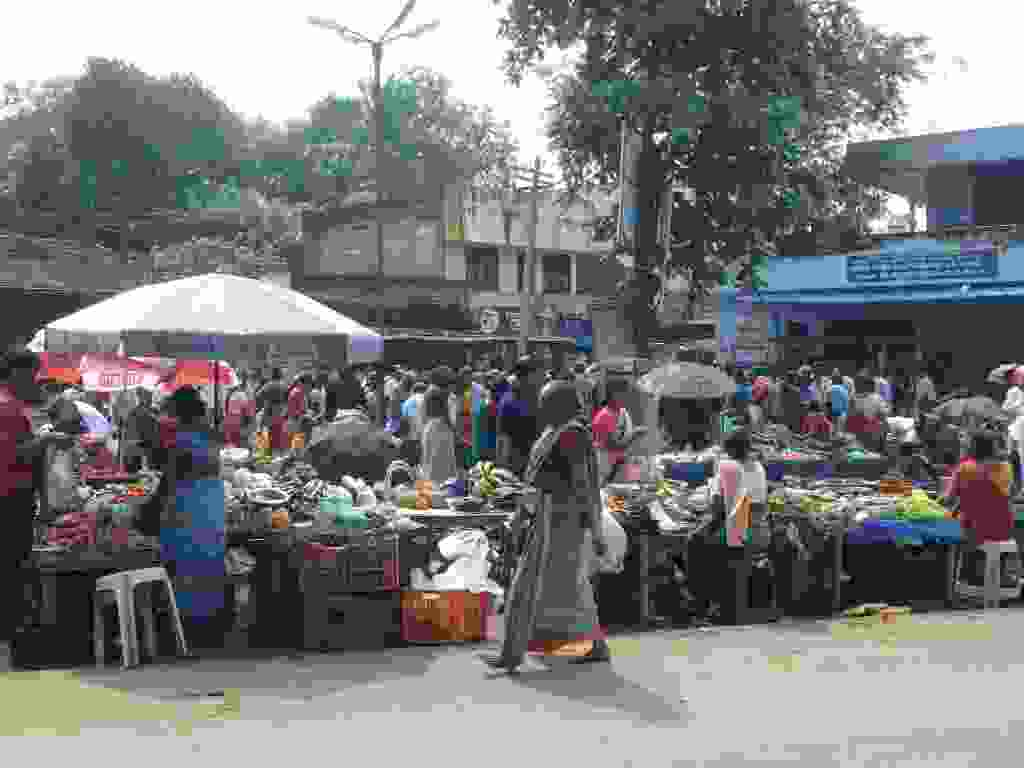
\includegraphics[width=\mywidth]{../wp-content/uploads/2015/11/PB110750-1024x768.jpg} \end{center}
\vspace{-\topsep}
\pagebreak

  Je m'arrête au temple de Swamithoppe. \\
\begin{center} 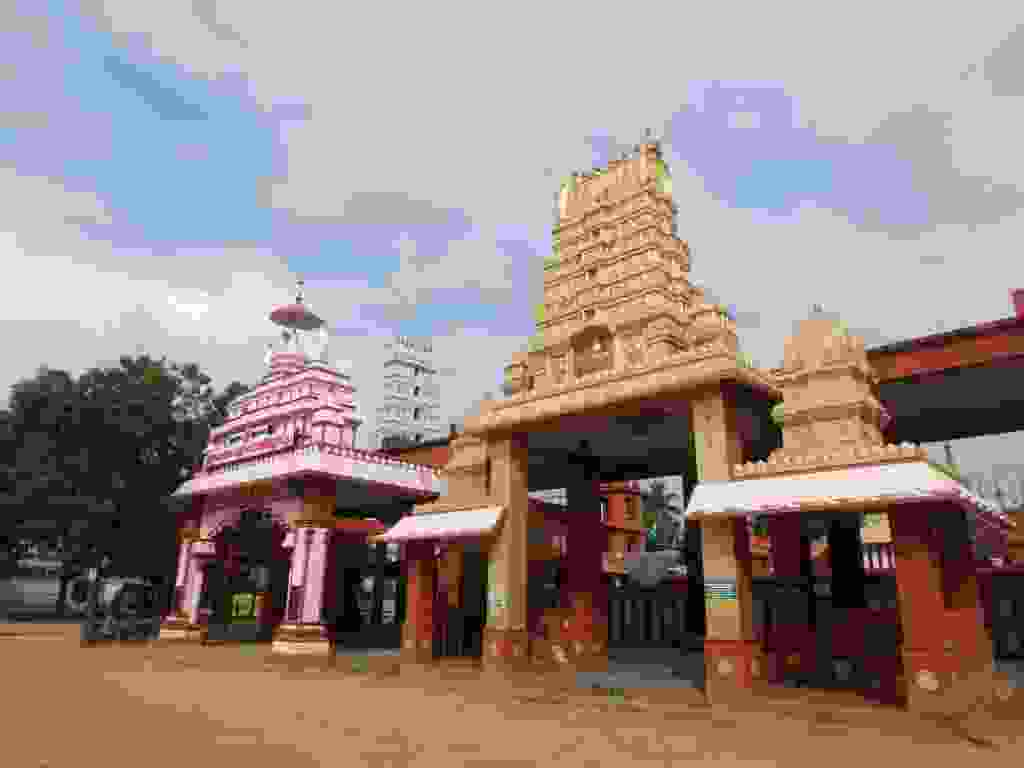
\includegraphics[width=\mywidth]{../wp-content/uploads/2015/11/PB110761-1024x768.jpg} \end{center}

 Quelques dizaines de personnes malades vivent dehors à côté du temple dans l'espoir d'une guérison. 
\begin{center} 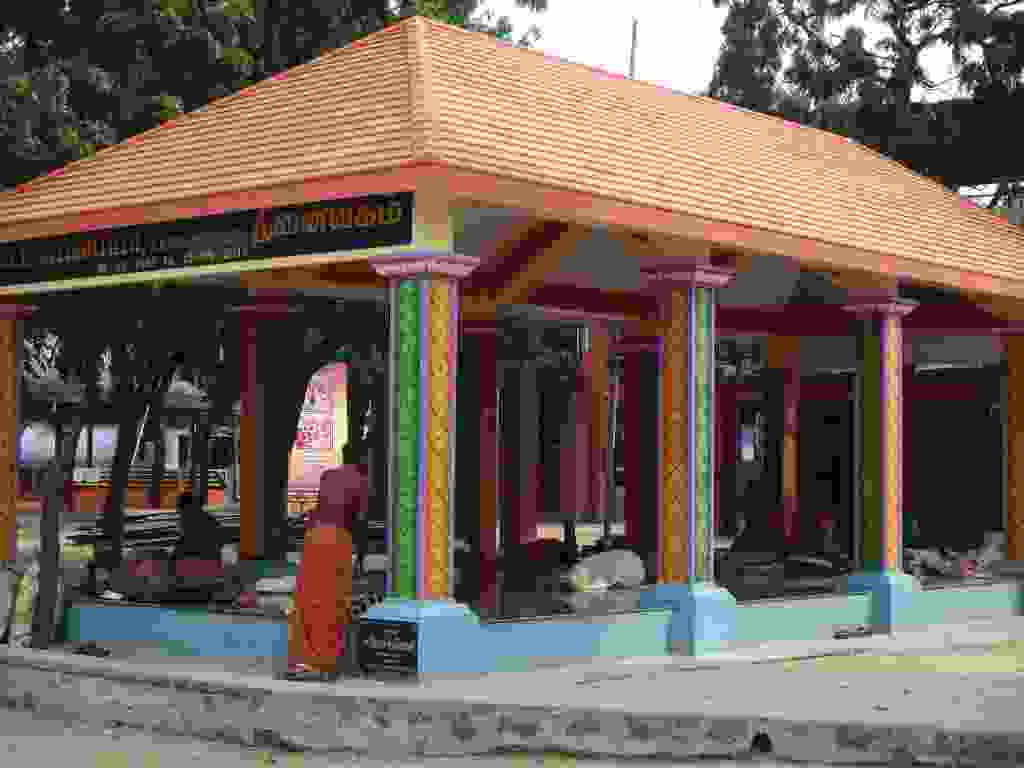
\includegraphics[width=\mywidth]{../wp-content/uploads/2015/11/PB110759-1024x768.jpg} \end{center}
\vspace{-\topsep}
\pagebreak
 
 Étape à Kanyakumari, une grande statue marque le point où se rejoignent les 3 mers : océan indien, golfe du Bengale et mer d'Arabie.
\begin{center} 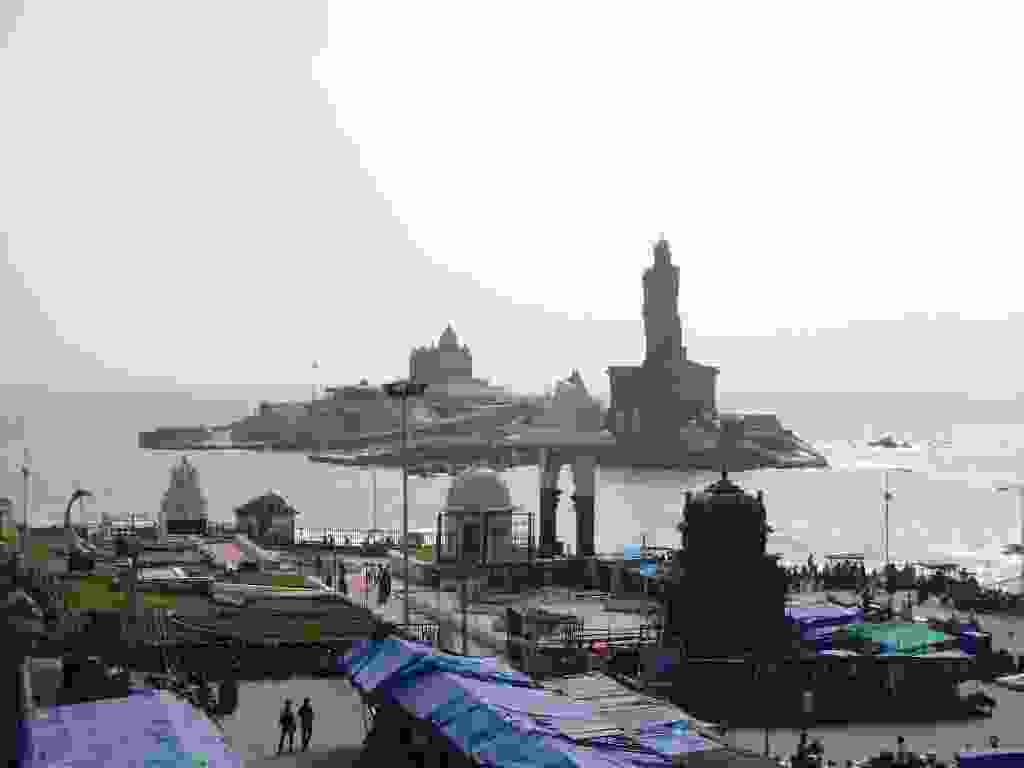
\includegraphics[width=\mywidth]{../wp-content/uploads/2015/11/PB120782-1024x768.jpg} \end{center}

 Mémorial de Gandhi. \\
\begin{center} 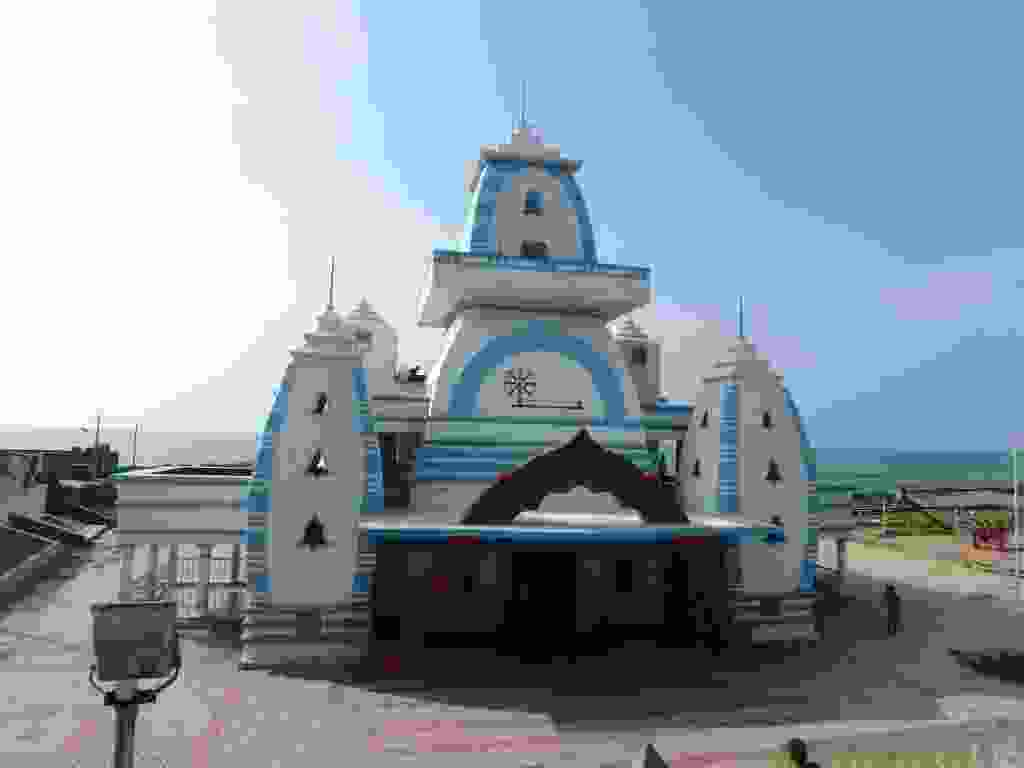
\includegraphics[width=\mywidth]{../wp-content/uploads/2015/11/PB120773-1024x768.jpg} \end{center}
\vspace{-\topsep}
\pagebreak
 
 Pour continuer vers le nord je choisis l'autoroute, très peu de trafic peut-être à cause du péage. 
\begin{center} 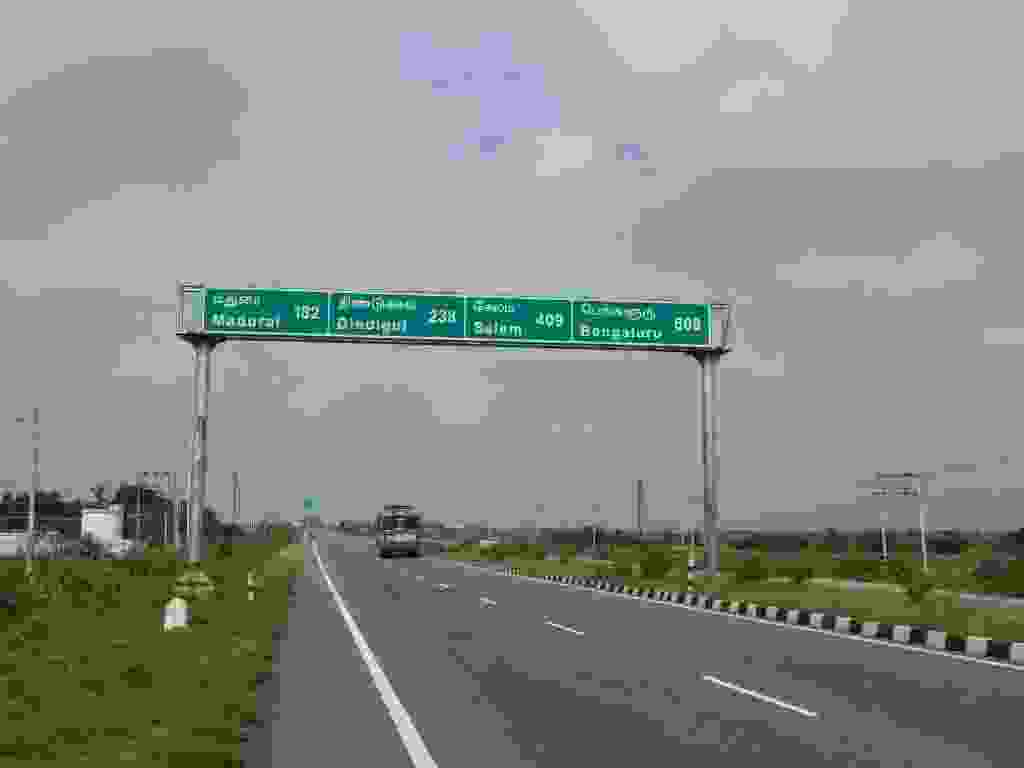
\includegraphics[width=\mywidth]{../wp-content/uploads/2015/11/PB120788-1024x768.jpg} \end{center}

 Étape à Tirunelveli. 
\begin{center} 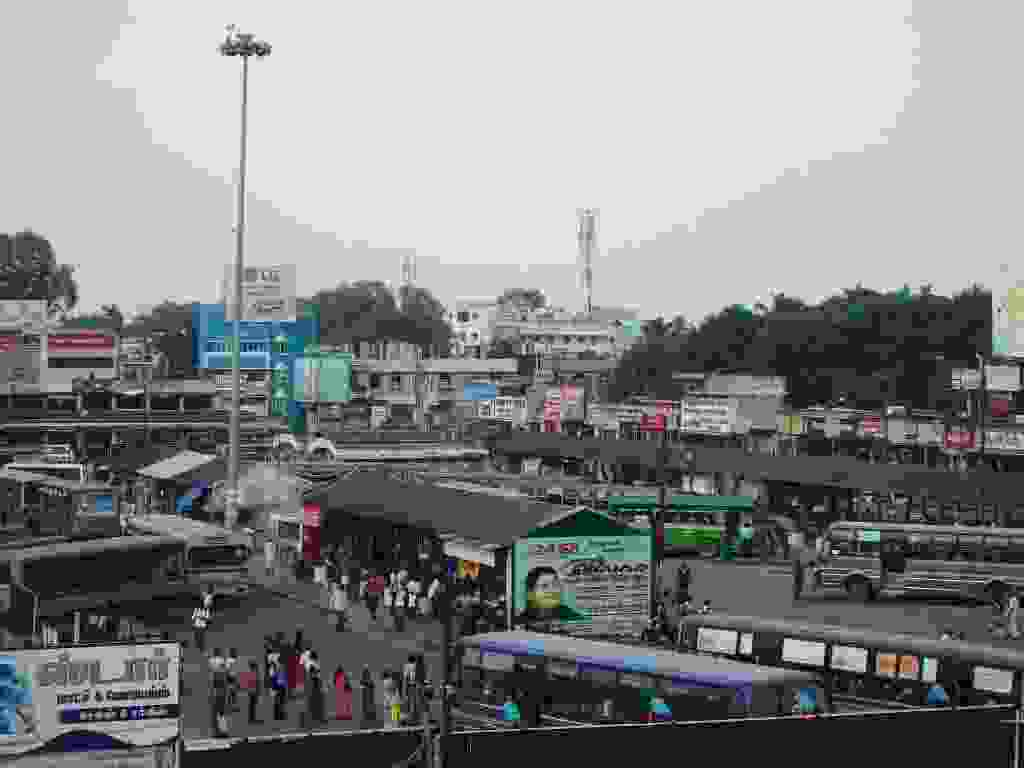
\includegraphics[width=\mywidth]{../wp-content/uploads/2015/11/wpid-oi000441-1024x768.jpg} \end{center}
\vspace{-\topsep}
\pagebreak

~\\
\vspace{0.5mm}
\begin{center} 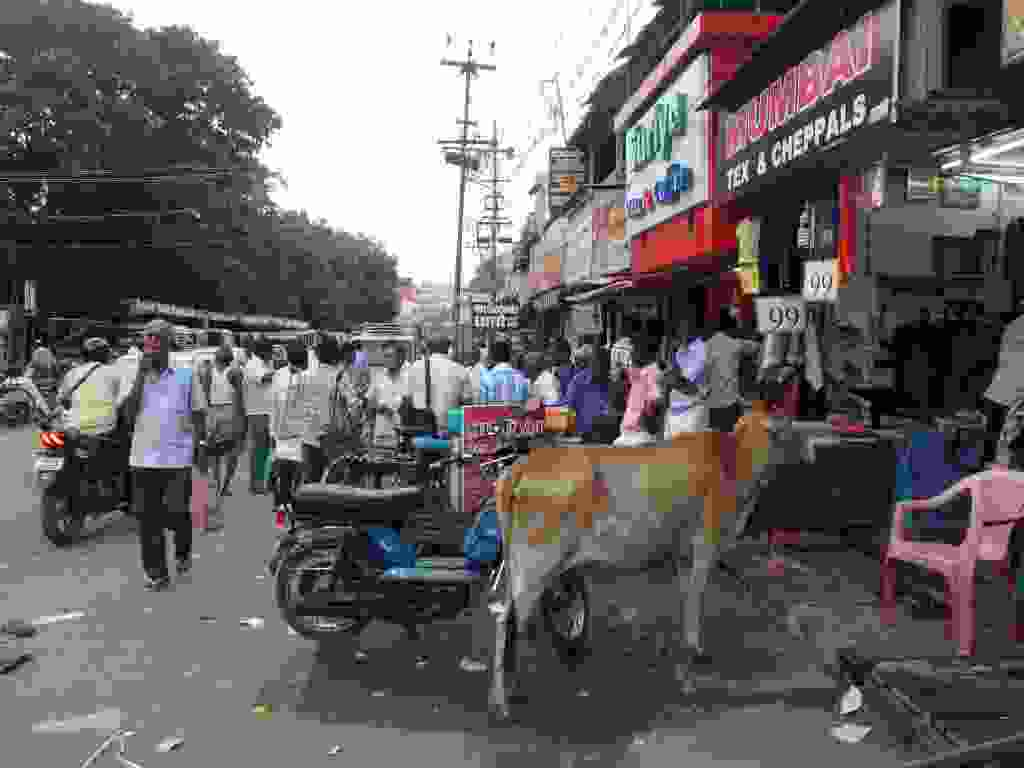
\includegraphics[width=\mywidth]{../wp-content/uploads/2015/11/PB120793-1024x768.jpg} \end{center}
~
\begin{center} 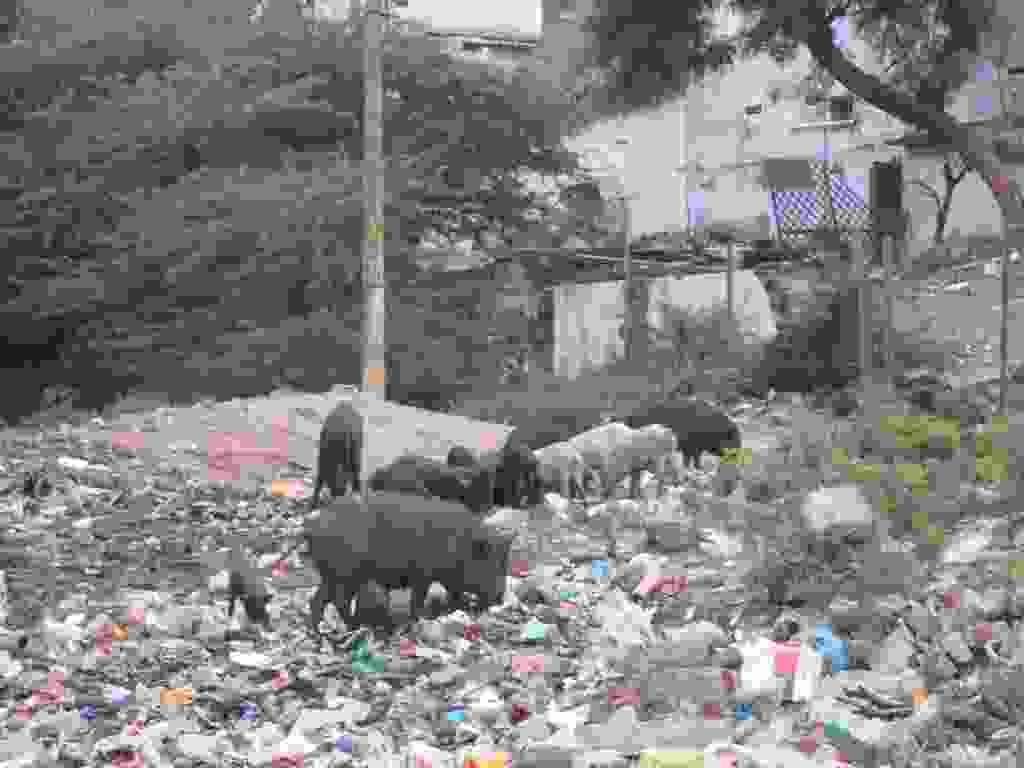
\includegraphics[width=\mywidth]{../wp-content/uploads/2015/11/PB120796-1024x768.jpg} \end{center}
\vspace{-\topsep}
\pagebreak
 
 Juste avant Madurai je suis malade à cause de la nourriture, je fais les derniers km en train. 
\begin{center} 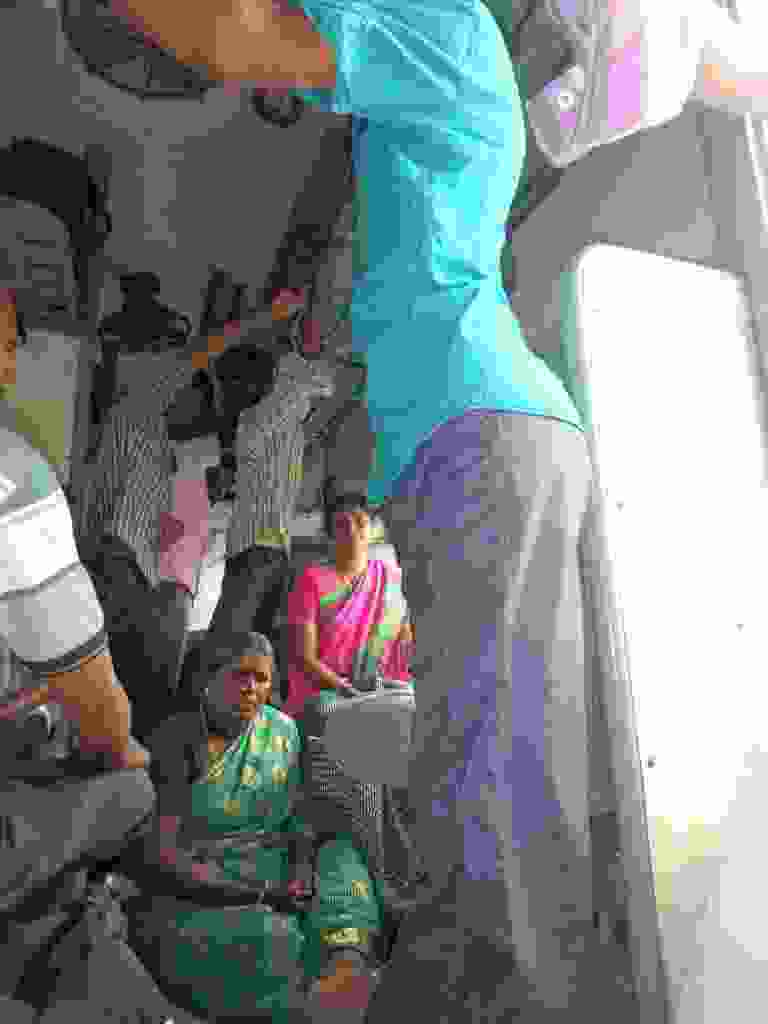
\includegraphics[height=0.75\textwidth]{../wp-content/uploads/2015/11/wpid-oi0002673-768x1024.jpg} \end{center}

 À Madurai, Karthik m'accueille dans sa belle maison et m'aide à me remettre d'aplomb. 
\begin{center} 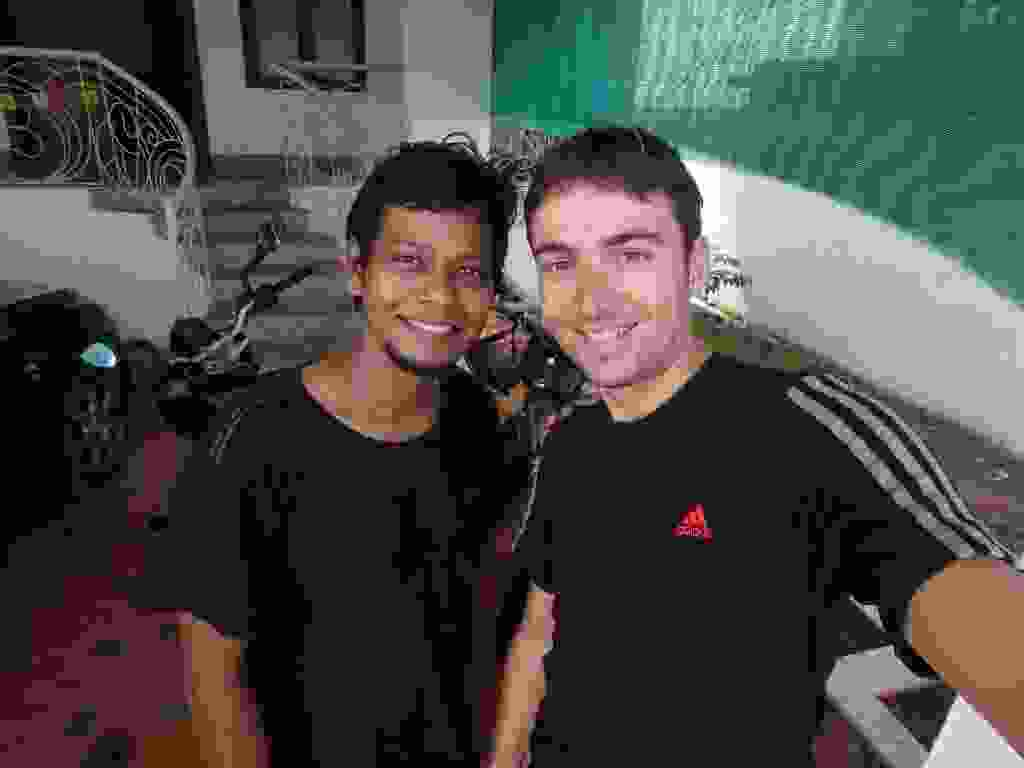
\includegraphics[width=\mywidth]{../wp-content/uploads/2015/11/wpid-oi000459-1024x768.jpg} \end{center}

 Temple Sri Meenakshi, grand et très fréquenté. Pas d'appareil photo et accès au sanctuaire central fermé aux étrangers, en même temps il y a des dizaines de boutiques et de stands de nourriture à l'intérieur. 
\begin{center} 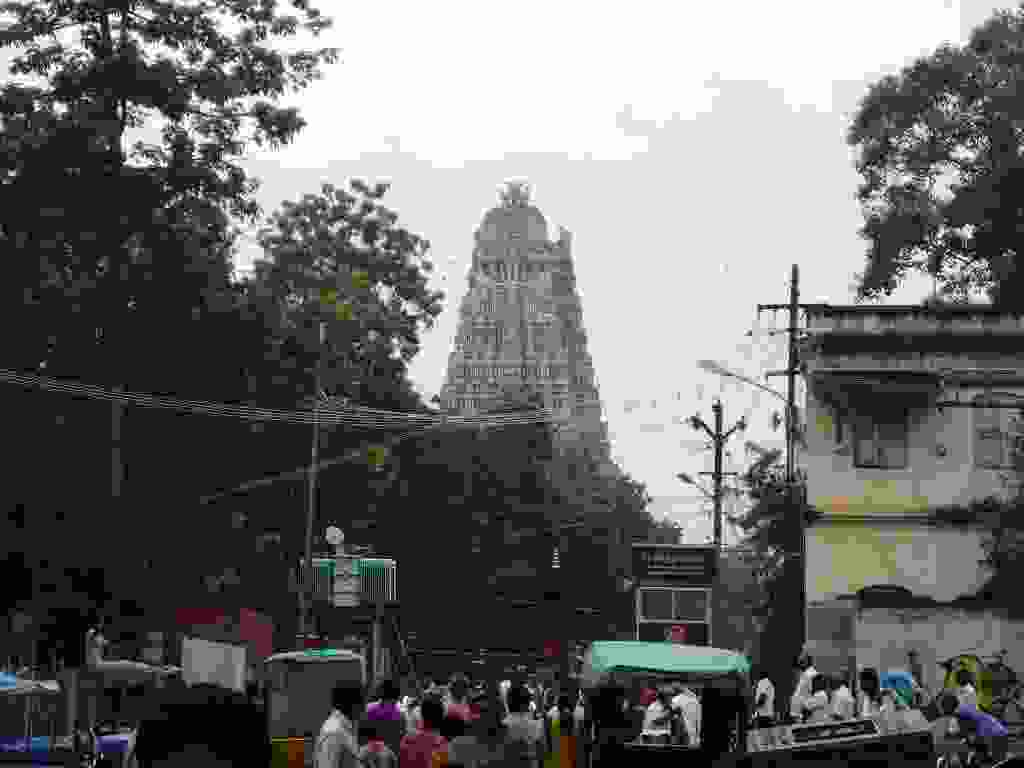
\includegraphics[width=\mywidth]{../wp-content/uploads/2015/11/wpid-oi0003731-1024x768.jpg} \end{center}
\begin{center} 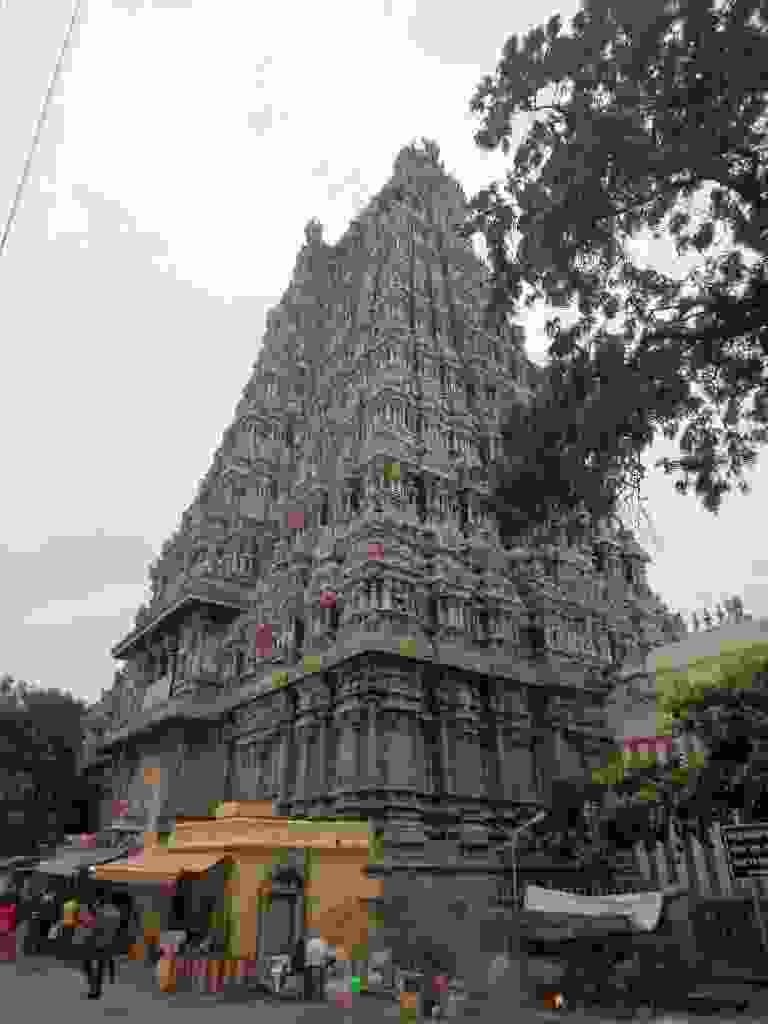
\includegraphics[height=0.8\textwidth]{../wp-content/uploads/2015/11/wpid-oi000455-e1448374927265-768x1024.jpg} \end{center}

  Palais Thirumalai Nayak. 
\begin{center} 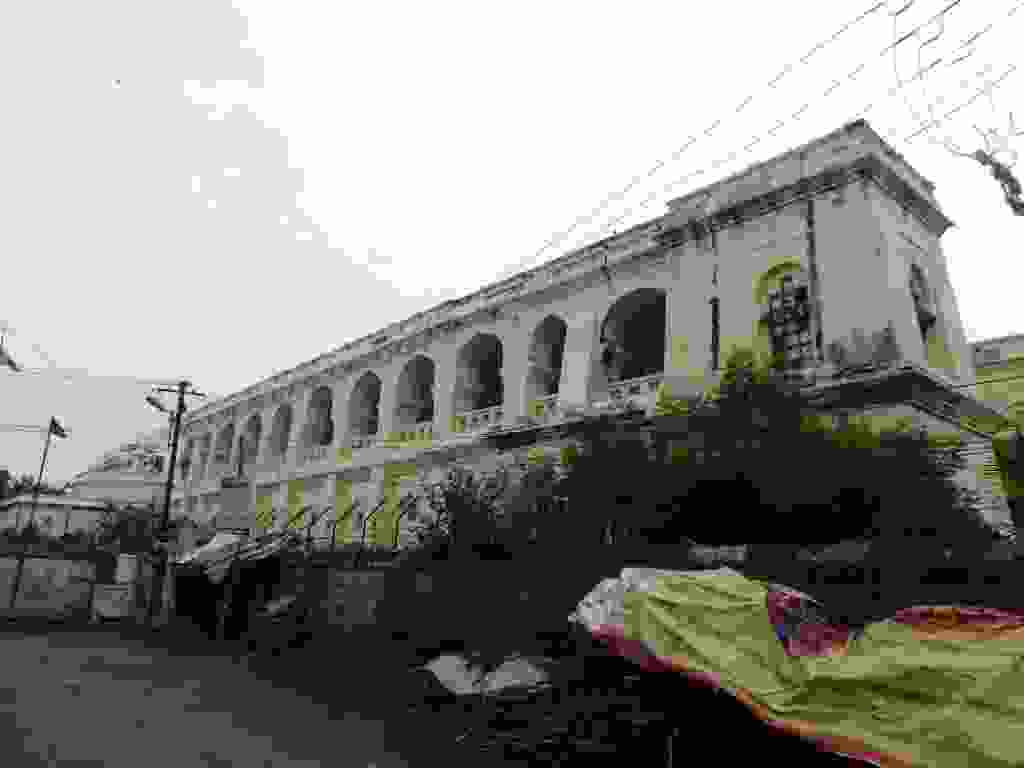
\includegraphics[width=\mywidth]{../wp-content/uploads/2015/11/PB150804-1024x768.jpg} \end{center}
~\\~\\
\begin{center} 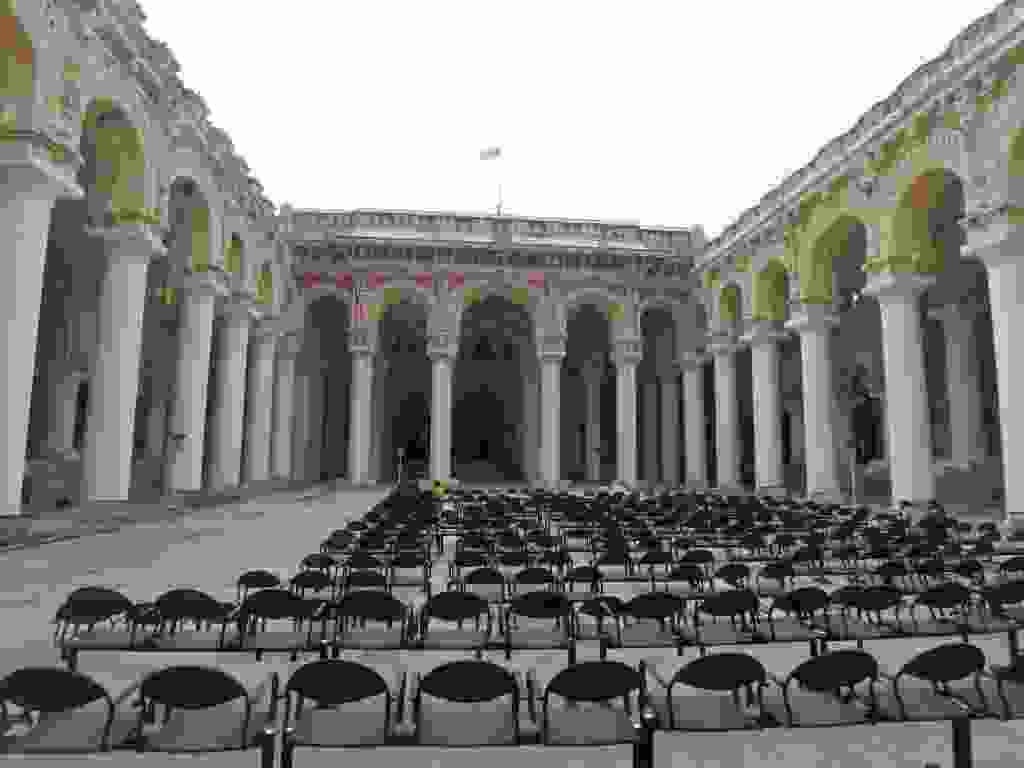
\includegraphics[width=\mywidth]{../wp-content/uploads/2015/11/PB150805-1024x768.jpg} \end{center}
\vspace{-\topsep}
\pagebreak

~
\vspace{0.75mm}
\begin{center} 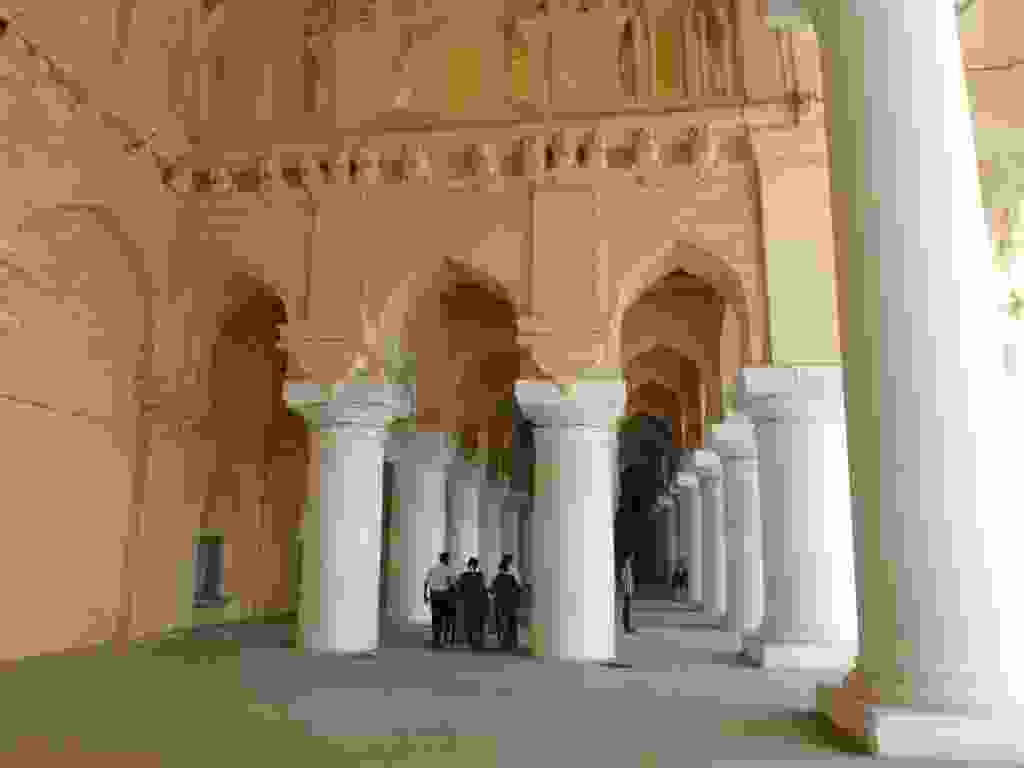
\includegraphics[width=\mywidth]{../wp-content/uploads/2015/11/PB150806-1024x768.jpg} \end{center}

 Je repars toujours vers le nord, je sens la différence entre Kerala et Tamil Nadu, terrain plus aride ici bien que les champs soient inondés pendant la saison des pluies. Les habitations sont plus simples aussi. 
\begin{center} 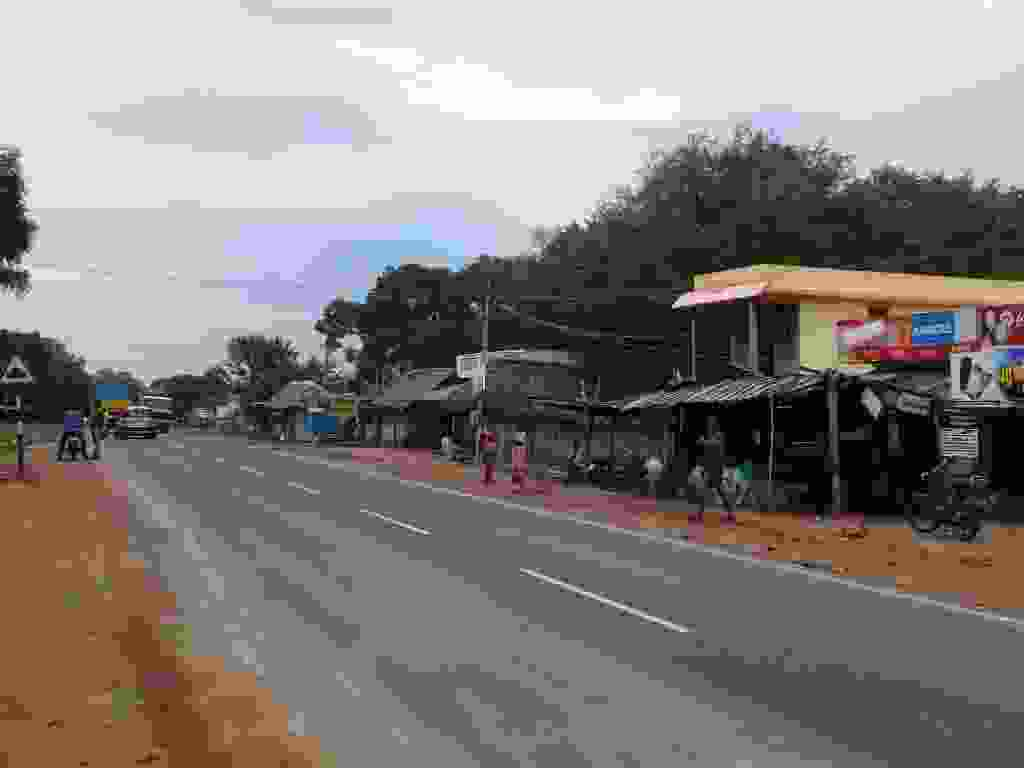
\includegraphics[width=\mywidth]{../wp-content/uploads/2015/11/wpid-oi000468-1024x768.jpg} \end{center}
\vspace{-\topsep}
\pagebreak

~\\~\\
\vspace{-0.5mm}
\begin{center} 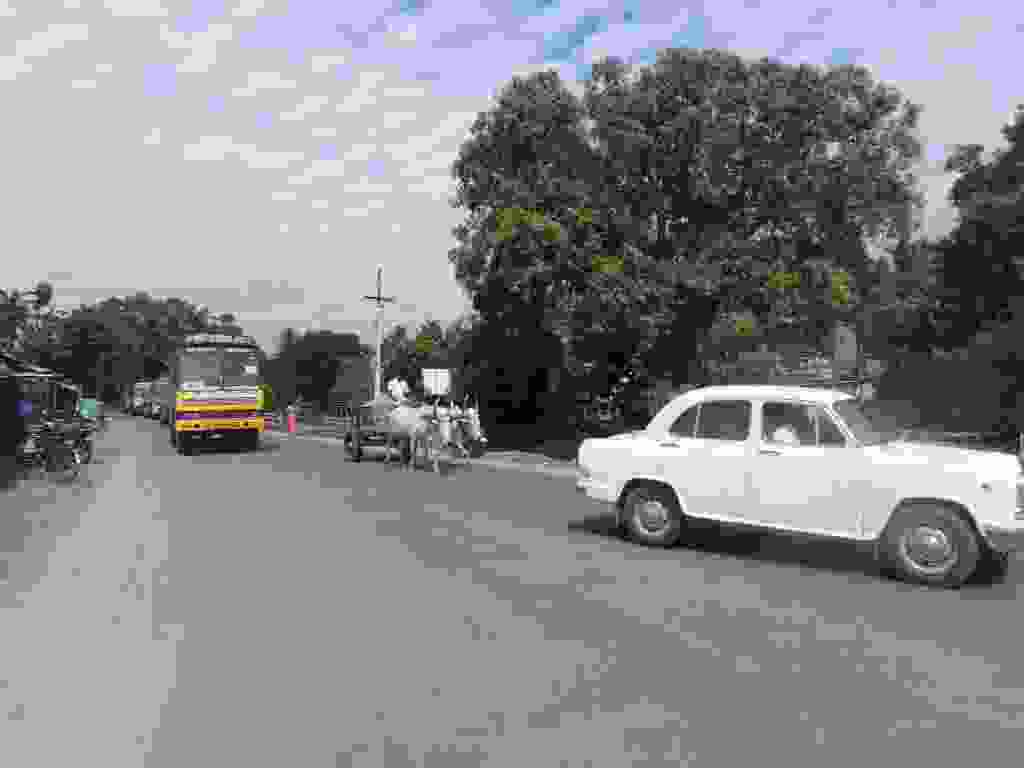
\includegraphics[width=\mywidth]{../wp-content/uploads/2015/11/wpid-oi000472-1024x768.jpg} \end{center}
\vfill
\begin{center} 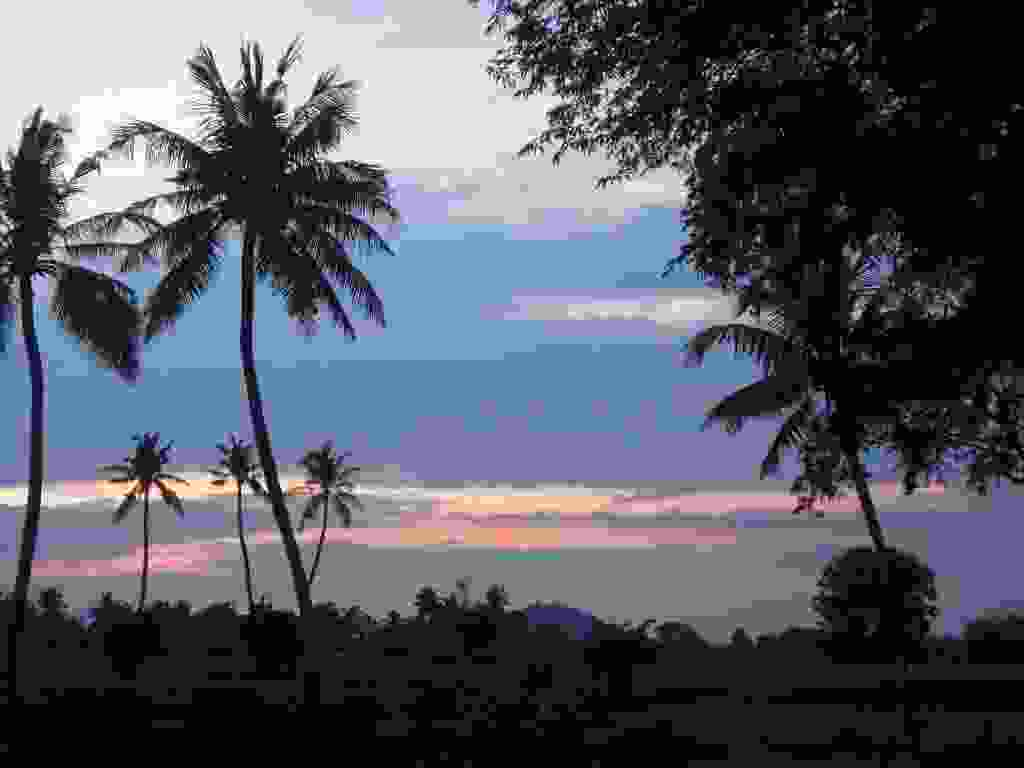
\includegraphics[width=\mywidth]{../wp-content/uploads/2015/11/wpid-oi000469-1024x768.jpg} \end{center}
\vspace{-\topsep}
\vspace{-0.75mm}
\pagebreak
 
 Sur la route vers Thanjavur, arrêt dans un petit ashram pour quelques jours au calme. Des visiteurs indiens ou européens sont là pour quelques jours ou semaines. 
\begin{center} 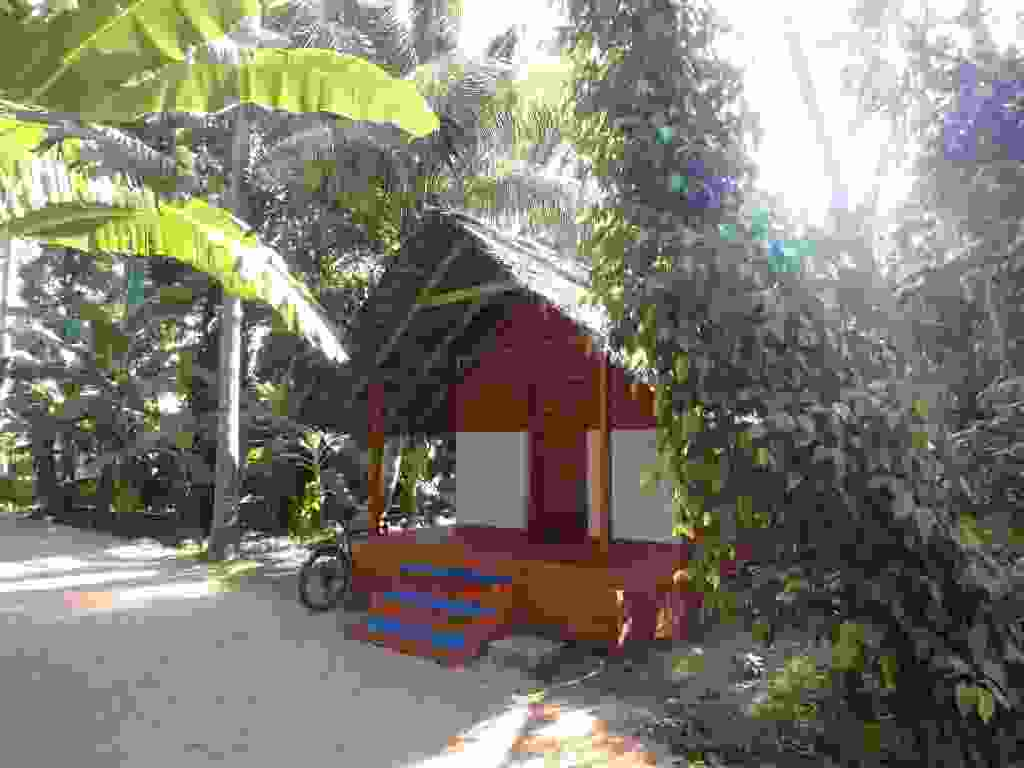
\includegraphics[width=\mywidth]{../wp-content/uploads/2015/11/wpid-oi000476-1024x768.jpg} \end{center}
\begin{center} 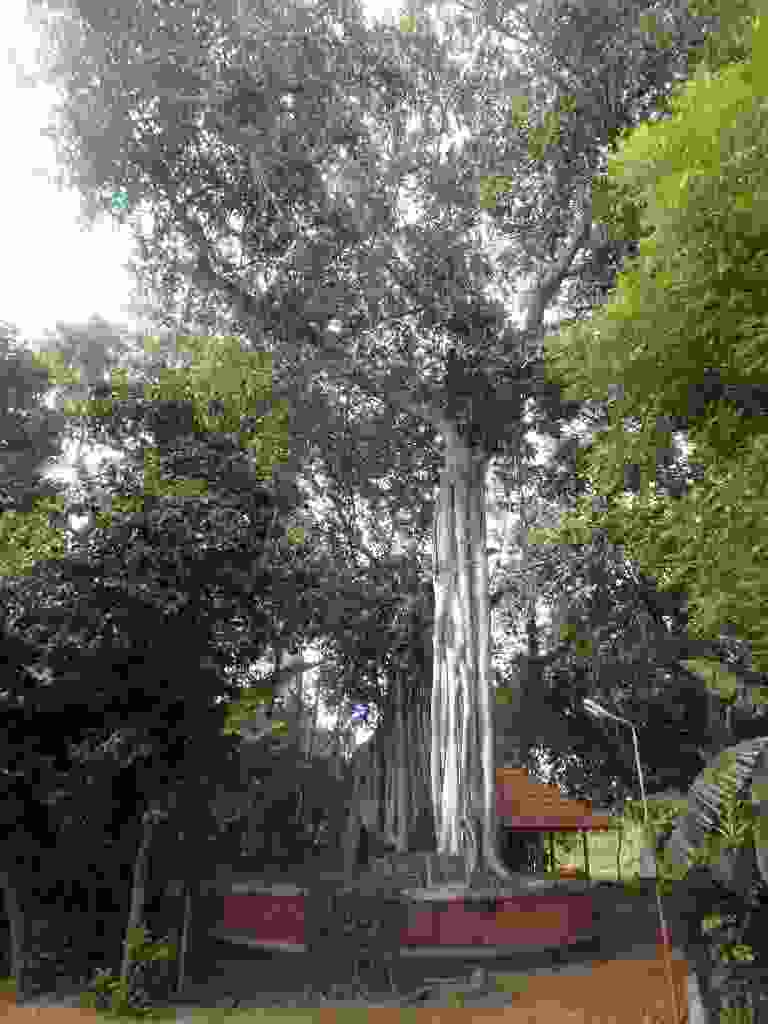
\includegraphics[height=0.8\textwidth]{../wp-content/uploads/2015/11/wpid-oi000478-e1448375113673-768x1024.jpg} \end{center}
\vspace{-\topsep}
\pagebreak

~
\begin{center} 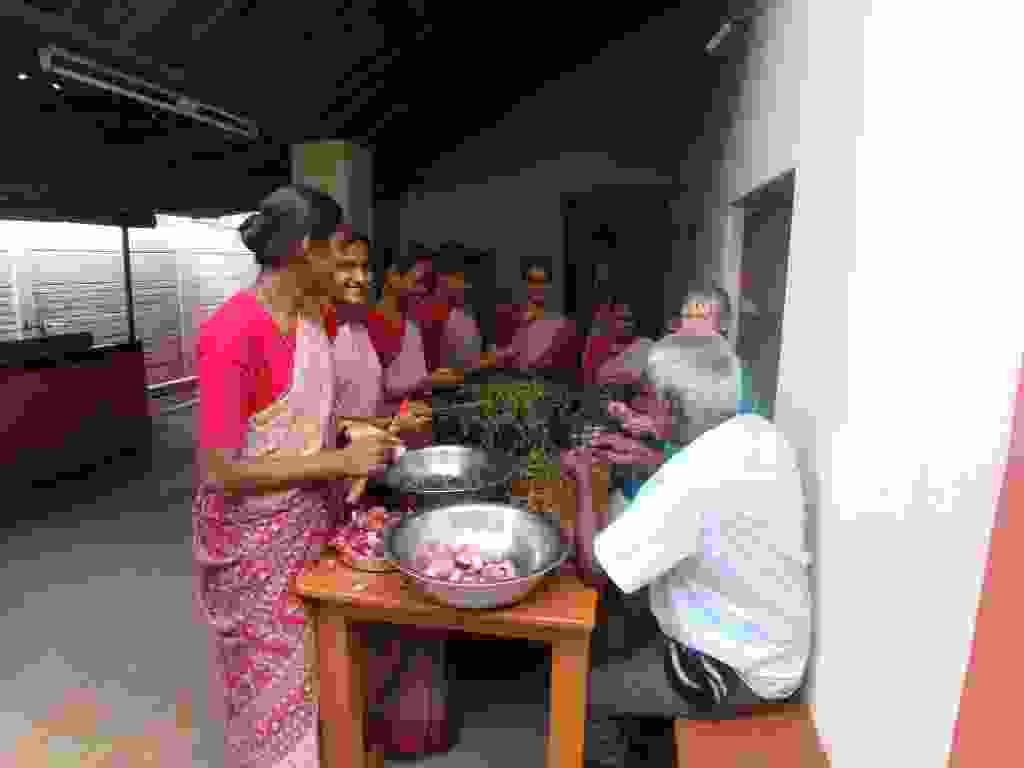
\includegraphics[width=\mywidth]{../wp-content/uploads/2015/11/wpid-oi00047201.jpg2-1024x768.jpg} \end{center}

  La nourriture de l'ashram. 
\begin{center} 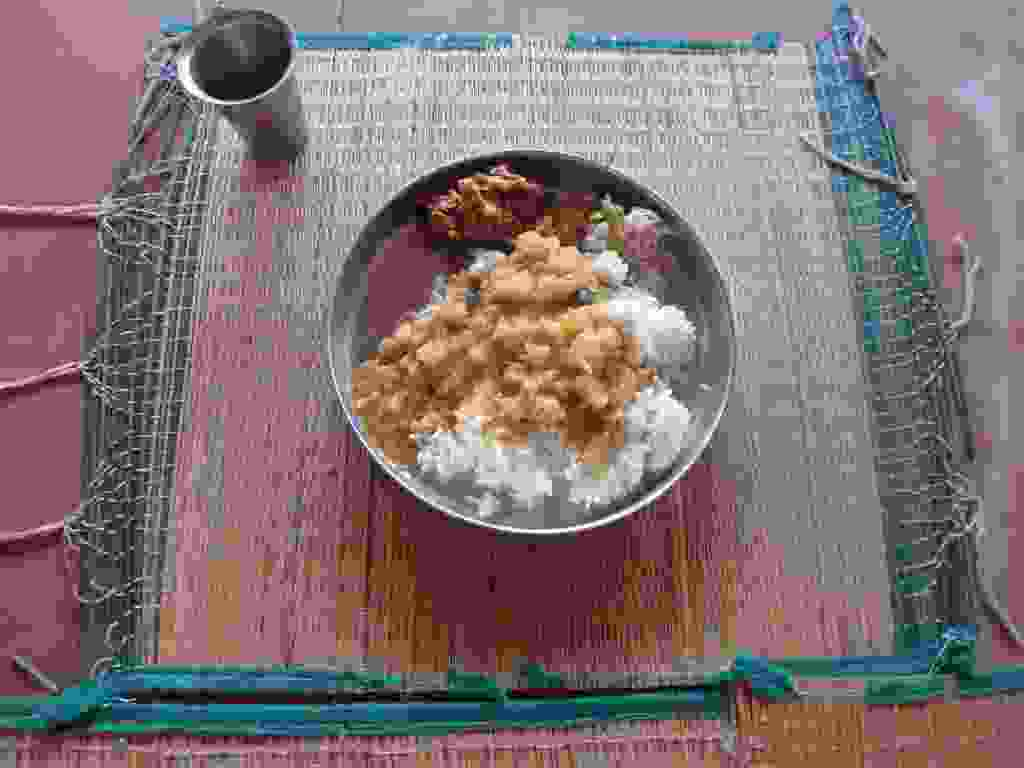
\includegraphics[width=\mywidth]{../wp-content/uploads/2015/11/wpid-oi00026701.jpg1-1024x768.jpg} \end{center}
\vspace{-\topsep}
\pagebreak
 
 Planning des journées, on peut choisir ce qu'on fait. 
\begin{center} 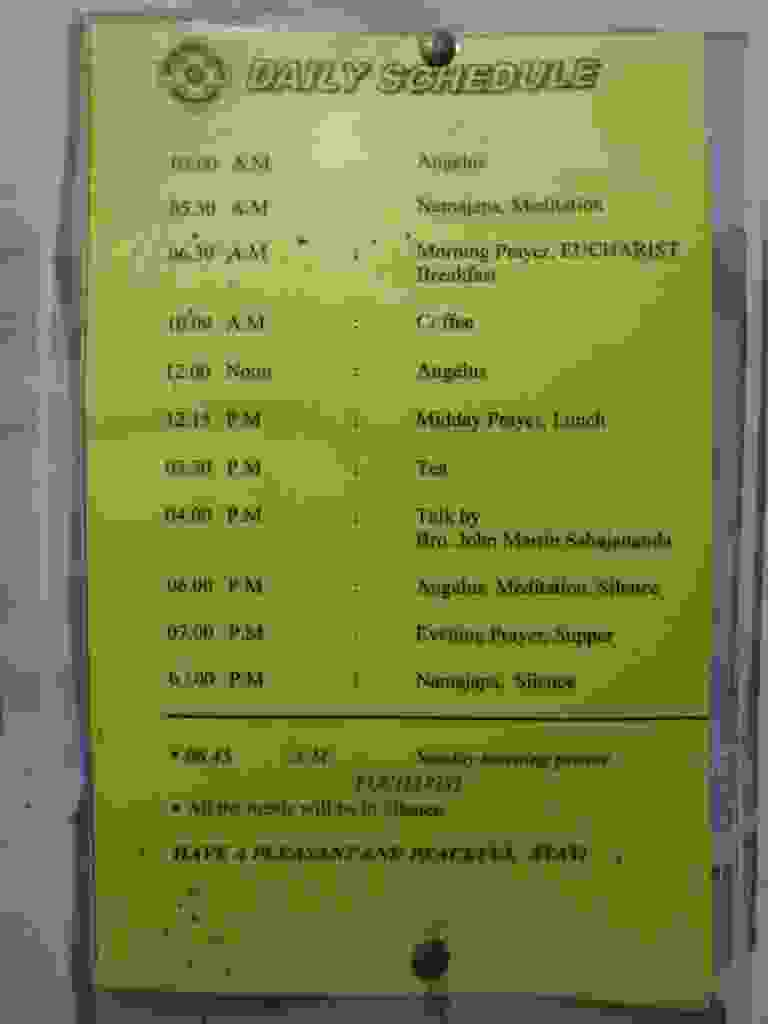
\includegraphics[height=0.82\textwidth]{../wp-content/uploads/2015/11/wpid-oi00037301.jpg1-e1448375246417-768x1024.jpg} \end{center}

 En passant à Trichy, je monte au Rockfort temple. 
\begin{center} 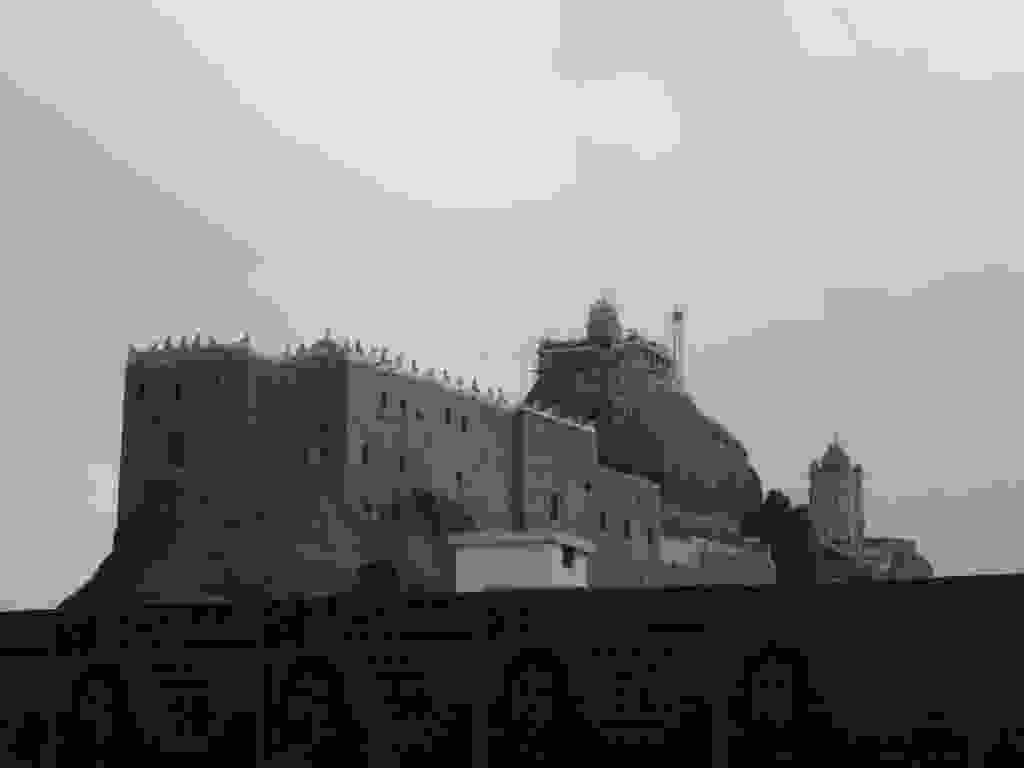
\includegraphics[width=\mywidth]{../wp-content/uploads/2015/11/wpid-oi0004892-1024x768.jpg} \end{center}
\begin{center} 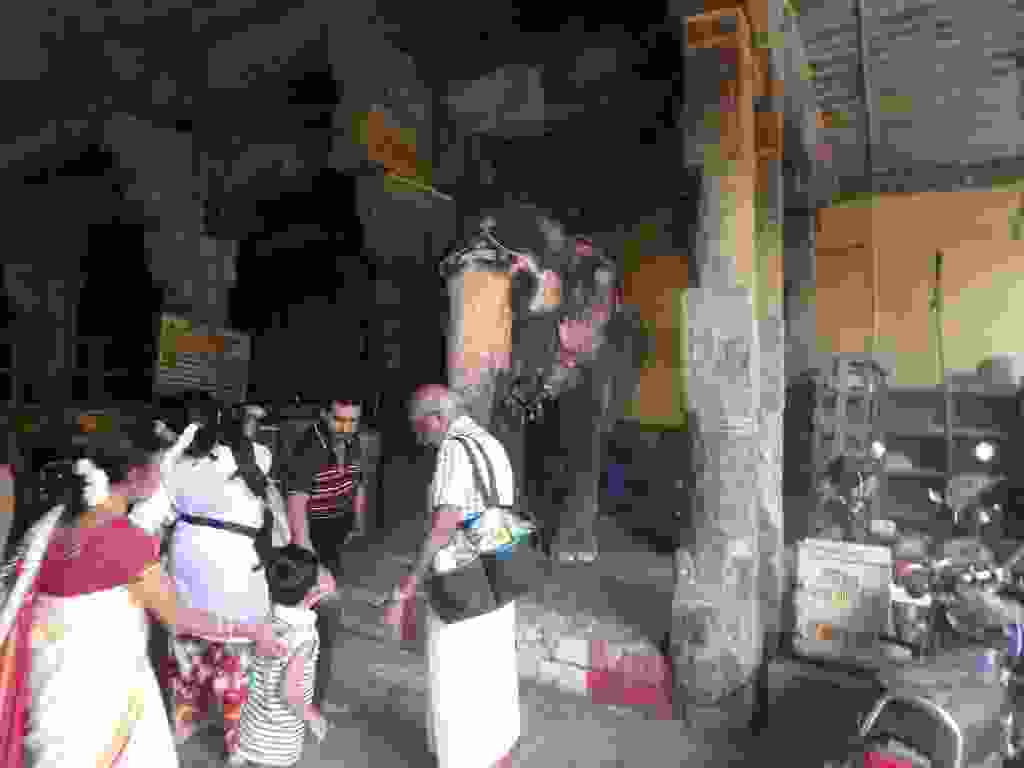
\includegraphics[width=\mywidth]{../wp-content/uploads/2015/11/wpid-oi0004902-1024x768.jpg} \end{center}
\begin{center} 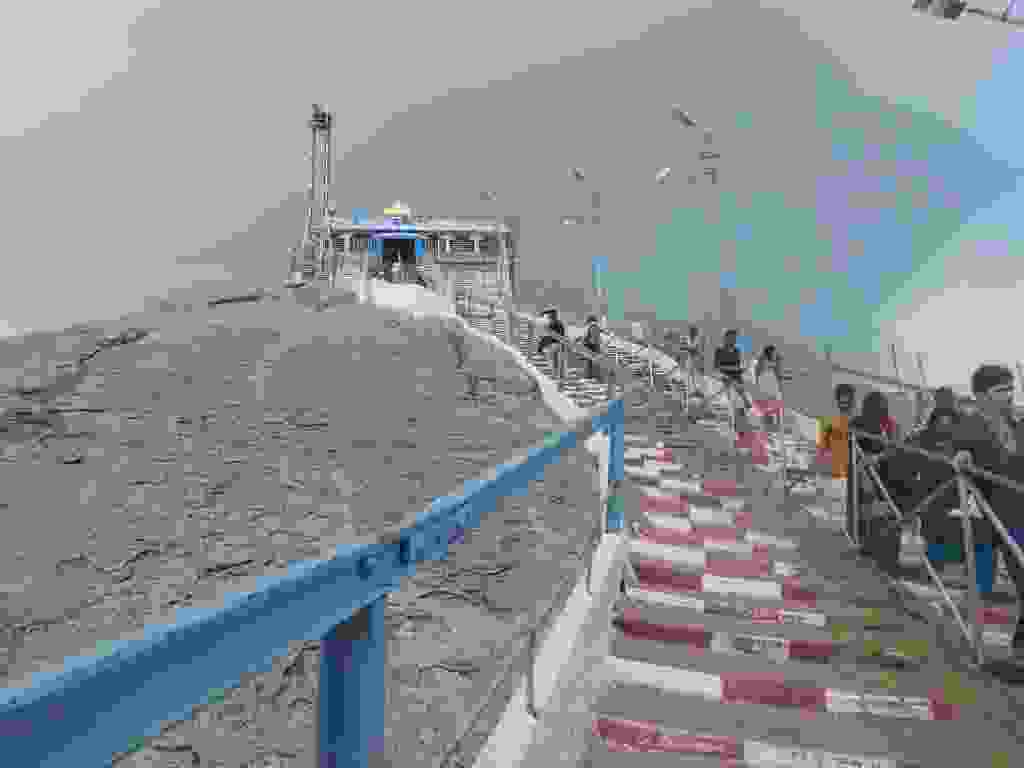
\includegraphics[width=\mywidth]{../wp-content/uploads/2015/11/wpid-oi0004911-1024x768.jpg} \end{center}
\begin{center} 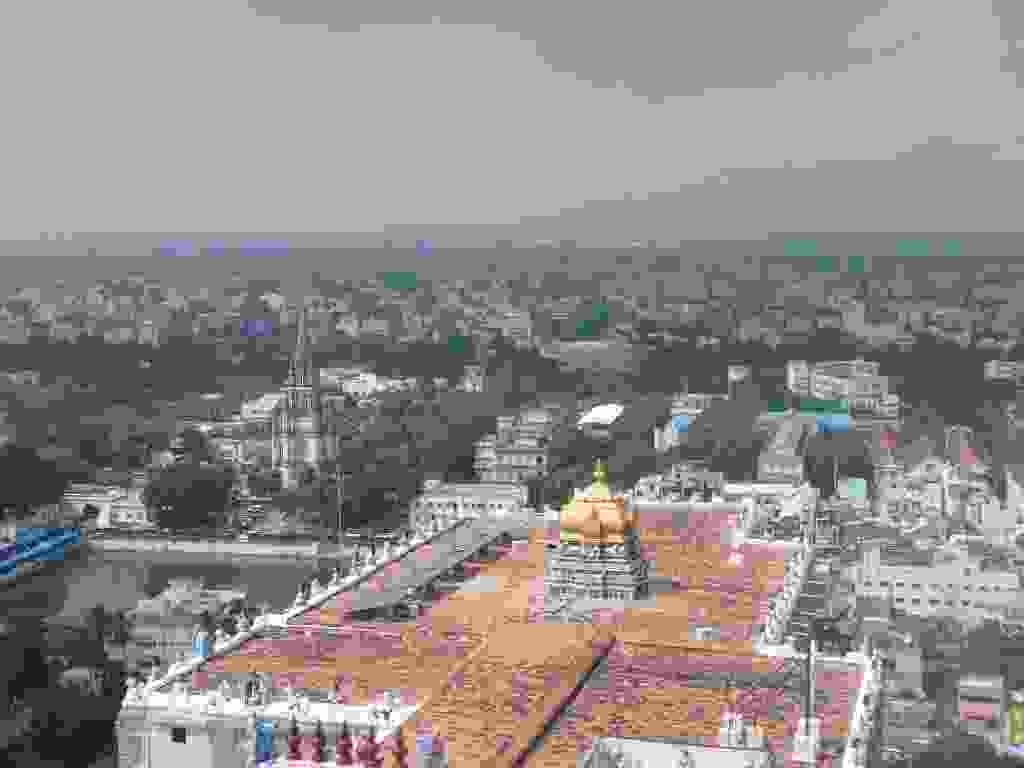
\includegraphics[width=\mywidth]{../wp-content/uploads/2015/11/wpid-oi0004941-1024x768.jpg} \end{center}

 Thanjavur et son superbe temple Brihadishwara, entrée gratuite et ici j'accède à toutes les parties du temple. 
\begin{center} 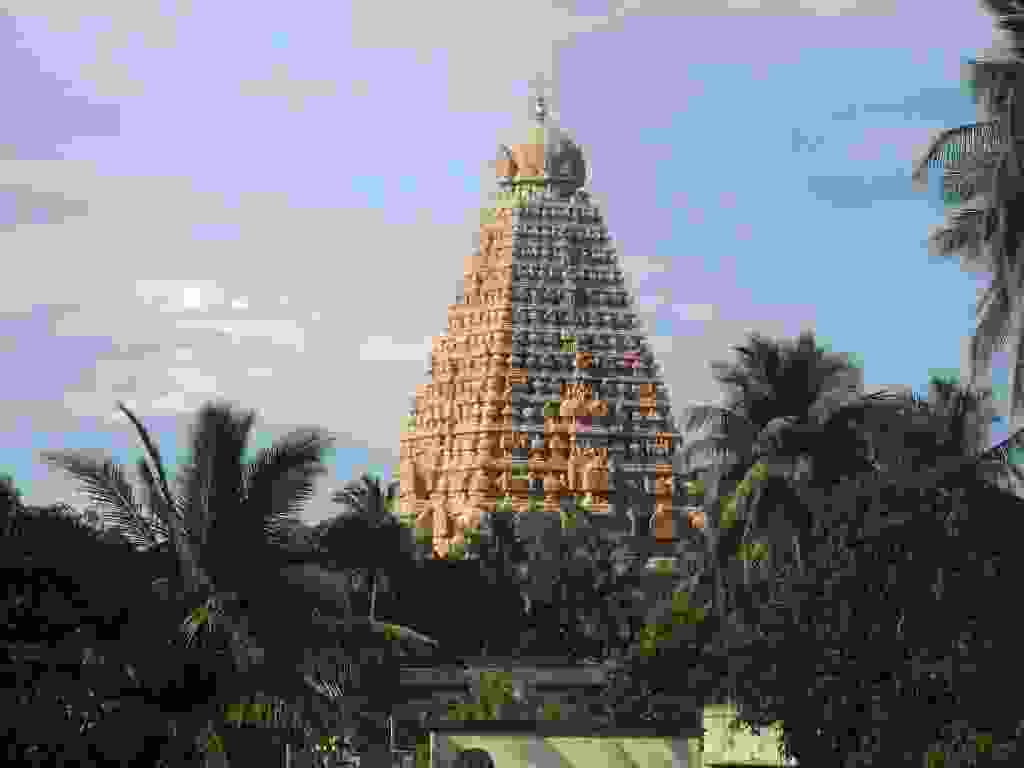
\includegraphics[width=\mywidth]{../wp-content/uploads/2015/11/wpid-oi000501-1024x768.jpg} \end{center}
\begin{center} 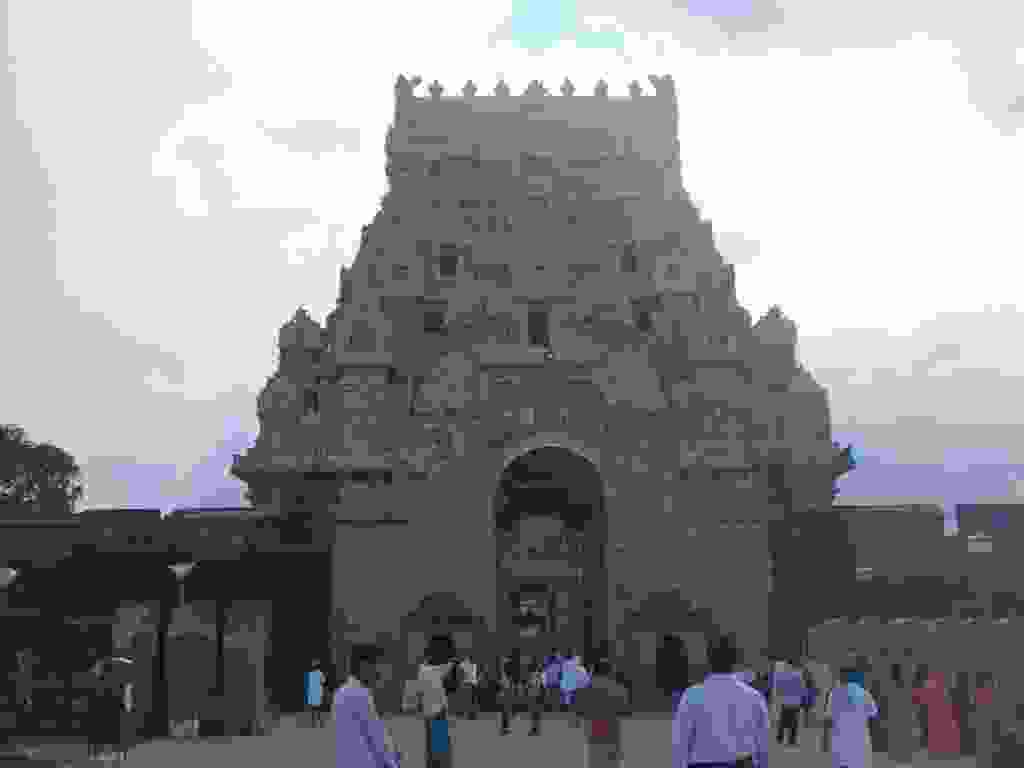
\includegraphics[width=\mywidth]{../wp-content/uploads/2015/11/wpid-oi000507-1024x768.jpg} \end{center}
\begin{center} 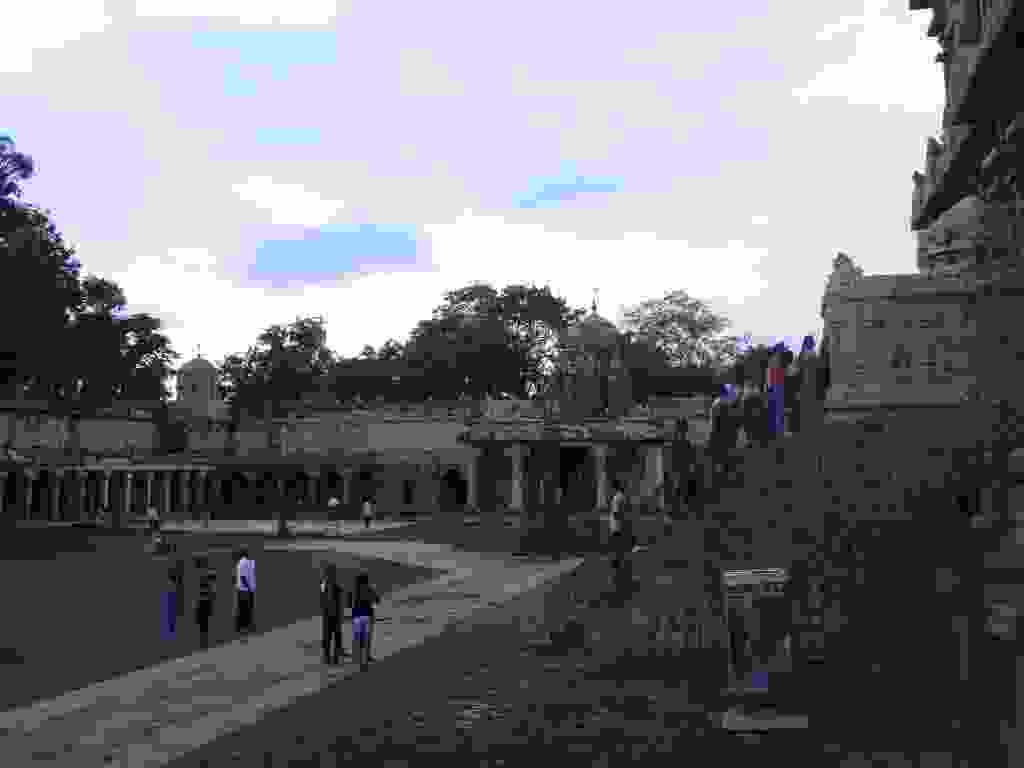
\includegraphics[width=\mywidth]{../wp-content/uploads/2015/11/wpid-oi000514-1024x768.jpg} \end{center}
\begin{center} 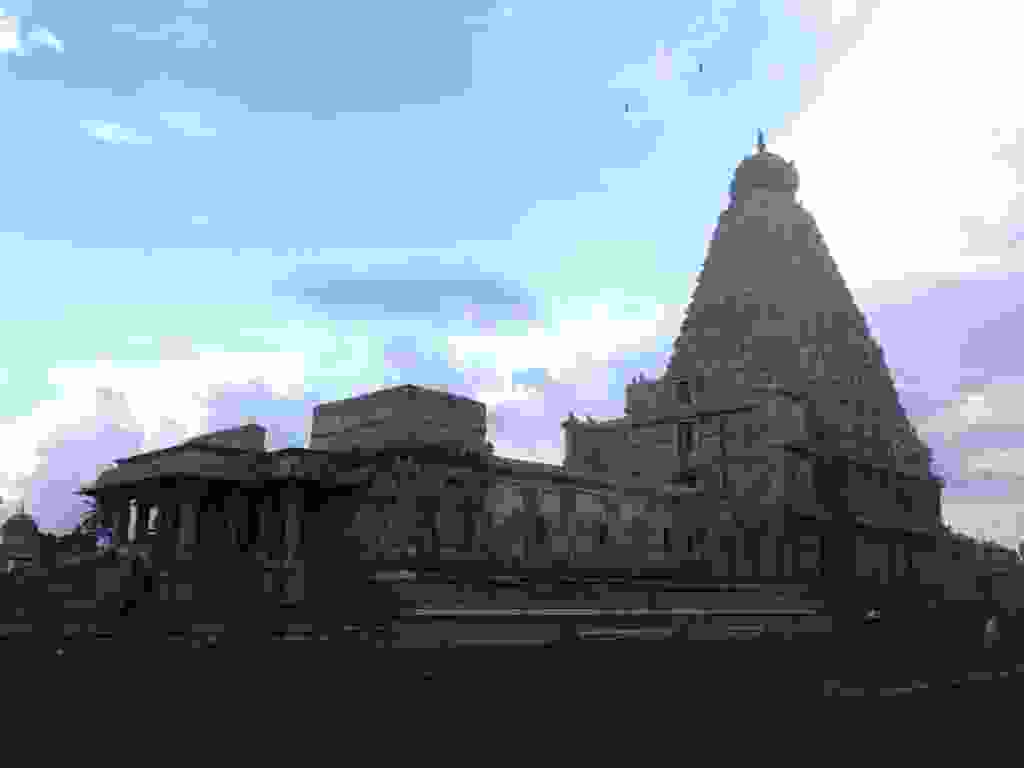
\includegraphics[width=\mywidth]{../wp-content/uploads/2015/11/wpid-oi000529-1024x768.jpg} \end{center}

 Palais de Thanjavur, pas très bien entretenu comme beaucoup de monuments par ici. 
\begin{center} 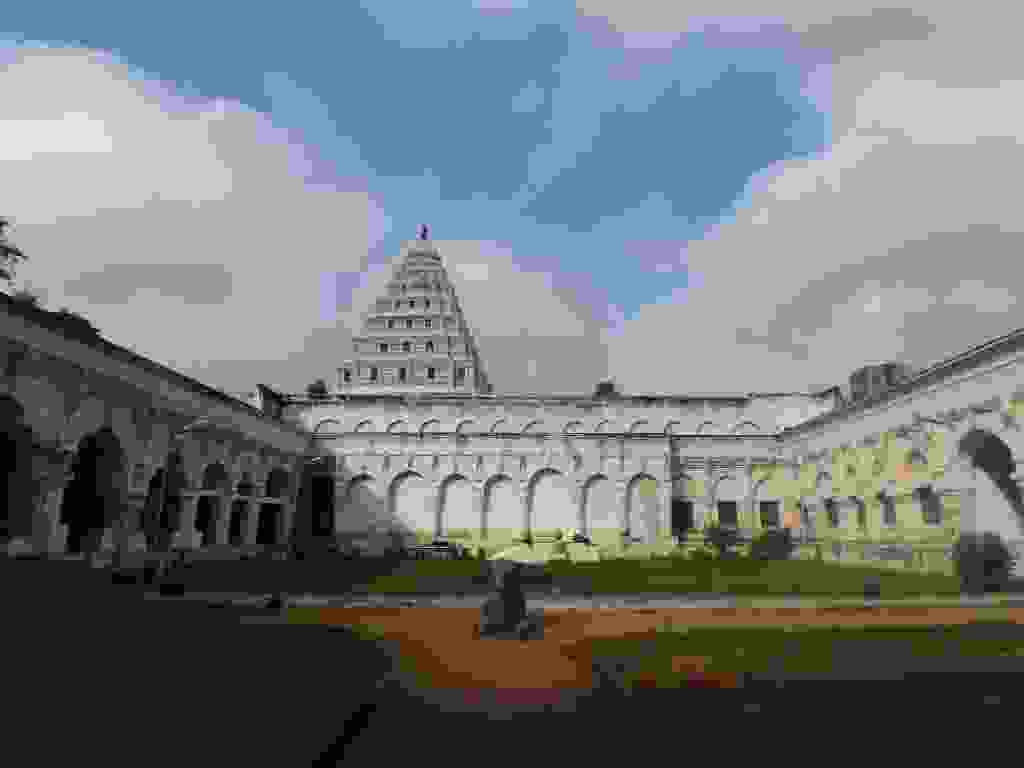
\includegraphics[width=\mywidth]{../wp-content/uploads/2015/11/wpid-oi000542-1024x768.jpg} \end{center}
\begin{center} 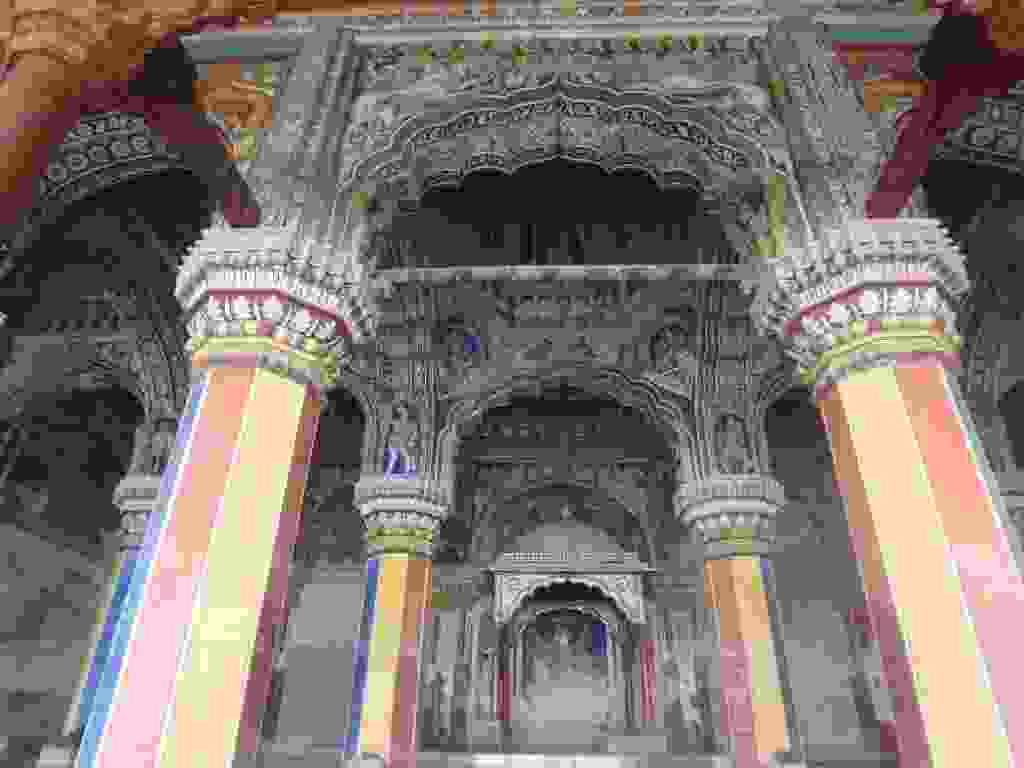
\includegraphics[width=\mywidth]{../wp-content/uploads/2015/11/wpid-oi000540-1024x768.jpg} \end{center}
\vspace{-\topsep}